\documentclass{ximera}
\input{../preamble.tex}

\author{D. Davis \and R. Speckert \and N. Shay \and A. Davis}
\title{Measurement, Data Collection and Represenatation} \license{CC BY-NC-SA 4.0}
\begin{document}

\begin{abstract}
\end{abstract}
\maketitle

\begin{onlineOnly}
\section*{Measurement, Data Collection and Represenatation}
\end{onlineOnly}

\begin{exploration}\label{exp:histogram1}
Consider a sample of 100 silicon wafers whose thickness of a metal layer resulting from a chemical vapor deposition (CVD) in a semiconductor plant. The data represent the layer thickness on semiconductor wafers measured in angstroms (one ten billionth of a meter).

% \begin{pdfOnly}
% Access GeoGebra interactives through the online version of this text at 

% \href{https://ximera.osu.edu/qcstats}{https://ximera.osu.edu/qcstats}.
% \end{pdfOnly}
CLICK on the SLIDER to change the number of buckets (bars).

\begin{onlineOnly}
\begin{center} 
\geogebra{dhvgryen}{800}{600} 
\end{center}
\end{onlineOnly}

We can see by the histogram output that the data has the triangular shape and symmetry associated with the bell shape. We can say that this sample data is normally distributed.


\end{exploration}

I'm including this wafer pic just for fun:

\begin{image}
         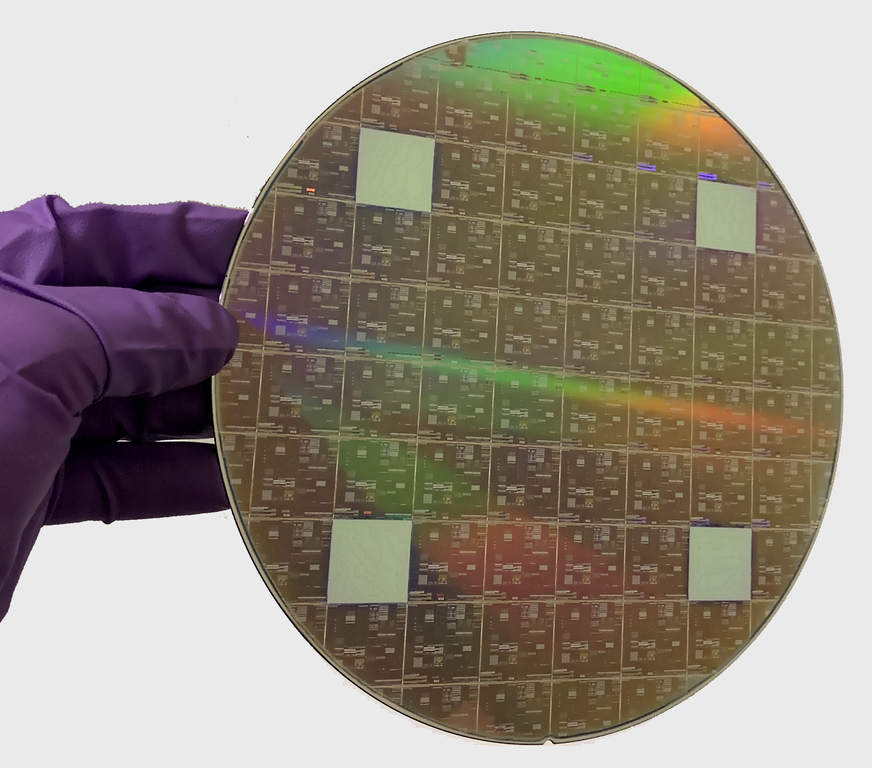
\includegraphics[height=1.5in]{200mmWafer.png}
\end{image}


\section*{Practice Problems}

\section*{References}
Wafer photo credit: \textit{Processed 200 mm Si Wafer} by Goldenvu CC BY-SA 4.0.

\end{document} 